\documentclass[10pt]{article}

\usepackage[a4paper]{geometry}
\usepackage[english]{babel}
\usepackage{array}
\usepackage{amsmath,amsthm,amsfonts,amssymb}
\usepackage{unicode}
\usepackage{subcaption}

\usepackage{algorithmic}
\renewcommand{\algorithmicrequire}{\textbf{Input:}}
\renewcommand{\algorithmicensure}{\textbf{Output:}}
\algsetup{linenodelimiter=.}

\usepackage{hyperref}
\hypersetup{
	unicode=true,
	colorlinks=true,
	citecolor=blue!70!black,
	filecolor=black,
	linkcolor=red!70!black,
	urlcolor=blue,
	pdfstartview={FitH},
}

\usepackage{tikz}
\usetikzlibrary{matrix,decorations,decorations.text,calc}
\pgfkeys{/triangle/.code=\tikzset{x={(-0.5cm,-0.866cm)},y={(1cm,0cm)}}}
\pgfkeys{/lattice/.code n args={4}{\tikzset{cm={#1,#2,#3,#4,(0,0)}}}}

\newcommand{\axes}[4]{
  \clip (#1,#3) rectangle (#2,#4);
  \draw [thin, gray, -latex] (#1,0) -- (#2,0);% Draw x axis
  \draw [thin, gray, -latex] (0,#3) -- (0,#4);% Draw y axis
}

\newcommand{\lattice}[3][2pt]{
  \draw[style=help lines,dashed] (#2-1,#2-1) grid[step=1] (#3+1,#3+1);
  \foreach \x in {#2,...,#3}{
    \foreach \y in {#2,...,#3}{
      \node[draw,circle,inner sep=#1,fill] at (\x,\y) {};
      % Places a dot at those points
    }
  }
}

% theorem environments
\theoremstyle{plain}
\newtheorem{theorem}{Theorem}
\newtheorem{lemma}[theorem]{Lemma}
\newtheorem{corollary}[theorem]{Corollary}
\newtheorem{proposition}[theorem]{Proposition}
\theoremstyle{definition}
\newtheorem{definition}[theorem]{Definition}
\newtheorem{example}[theorem]{Example}
\newtheorem{exercice}{Exercice}[section]

\DeclareMathOperator{\Aut}{Aut}
\DeclareMathOperator{\End}{End} % endomorphism ring
\DeclareMathOperator{\Tr}{Tr} % finite field trace
\DeclareMathOperator{\Gal}{Gal} % Galois group
\DeclareMathOperator{\ord}{ord} % order of an element
\DeclareMathOperator{\lcm}{lcm} % least common multiple
\DeclareMathOperator{\norm}{N} % norm
\DeclareMathOperator{\loglog}{loglog}
\DeclareMathOperator{\im}{Im}
\DeclareMathOperator{\GL}{GL}
\DeclareMathOperator{\SL}{SL}

\def\A{\ensuremath{\mathbb{A}}}
\def\P{\ensuremath{\mathbb{P}}}
\def\F{\ensuremath{\mathbb{F}}}
\def\O{\ensuremath{\mathcal{O}}}
\def\euler{\ensuremath{\varphi}}

\title{Isogeny Based Cryptography}
\author{Luca De Feo\\
  Universit\'e de Versailles \& Inria Saclay\\
  \url{http://defeo.lu/}}
\date{\'Ecole math\'ematique africaine\\
  May 10 -- 23, 2017, Thi\`es, Senegal}

\begin{document}
\maketitle

\section*{Introduction}

These lectures notes were written for a summer school on
\emph{Mathematics for Post-quantum cryptography} in Thiès, Senegal. %
They try to provide a guide for Masters' students to get through the
vast literature on elliptic curves, without getting lost on their way
to learning isogeny-based cryptography. %
They are by no means a reference text on the theory of elliptic
curves, nor on cryptography; students are encouraged to complement
these notes with some of the books recommended in the bibliography. %

The presentation is divided in three sections, roughly corresponding
to the three lectures given. %
In an effort to keep the reader interested, each sections alternates
between the fundamental theory of elliptic curves, and applications in
cryptography. %
We often prefer to have the main ideas flow smoothly, rather than
having a rigorous presentation as one would have in a more classical
book. %
The reader will excuse us for the inaccuracies and the omissions.

\paragraph{Isogeny Based Cryptography} is a very young field, that has
only begun in the 2000s. %
It has its roots in \emph{Elliptic Curve Cryptography} (ECC), a
somewhat older branch of public-key cryptography that was started in
the 1980s, when Miller and Koblitz first suggested to use elliptic
curves inside the Diffie-Hellman key exchange protocol (see
Section~\ref{sec:appl-diff-hellm}). %

ECC only started to gain traction in the 1990s, after Schoof's
algorithm made it possible to easily find elliptic curves of large
prime order. %
It is nowadays a staple in public-key cryptography. %
The 2000s have seen two major innovations in ECC: the rise of
\emph{Pairing Based Cryptography} (PBC), epitomized by Joux' one-round
tripartite Diffie-Hellman key exchange, and the advent of
Isogeny-based cryptography, initiated by the works of Teske and
Rostovtsev \& Stolbunov. %
While PBC has attracted most of the attention during the first decade,
thanks to its revolutionary applications, isogeny based cryptography
has stayed mostly discrete during this time. %
It is only in the second half of the 2010 that the attention has
partly shifted to isogenies. %
The main reason for this is the sudden realization by the
cryptographic community of the very possibly near arrival of a
\emph{general purpose quantum computer}. %
While the capabilities of such futuristic machine would render all ECC
and PBC suddenly worthless, isogeny based cryptography seems to resist
much better to the cryptanalytic powers of the quantum computer.

In these notes, after a review of the general theory of elliptic
curves and isogenies, we will present the most important isogeny-based
systems, and their cryptographic properties.


%%%%%%%%%%%%%%%%%%%%%%%%%%%%%%%%%%%%%%%%%%%%%%%%%%%%%%

\section{Elliptic curves and cryptography}

Throughout this section we let $k$ be a field, and we denote by
$\bar{k}$ its algebraic closure. %
We review the basic theory of elliptic curves, and two classic
applications in cryptography. %
The interested reader will find more details on elliptic curves
in~\cite{silverman:elliptic}, and on their use in cryptography
in~\cite{joux2009algorithmic,galbraith2012mathematics}.

\subsection{Elliptic curves}

Elliptic curves are projective curves of genus 1 having a specified
base point. %
Projective space initially appeared through the process of adding
\emph{points at infinity}, as a method to understand the geometry of
projections (also known as \emph{perspective} in classical
painting). %
In modern terms, we define projective space as the collection of all
lines in affine space passing through the origin.

\begin{definition}[Projective space]
  The \emph{projective space of dimension $n$}, denoted by $\P^n$ or
  $\P^n(\bar{k})$, is the set of all $(n+1)$-tuples
  \[(x_0,\dots,x_n) ∈ \bar{k}^{n+1}\] %
  such that $(x_0,\dots,x_n) ≠ (0,\dots,0)$, taken modulo the
  equivalence relation
  \[(x_0,\dots,x_n) \sim (y_0,\dots,y_n)\] %
  if and only if there exists $λ\in\bar{k}$ such that
  $x_i=λ_iy_i$ for all $i$.
\end{definition}

The equivalence class of a projective point $(x_0,\dots,x_n)$ is
customarily denoted by $(x_0:\cdots:x_n)$. %
The set \emph{$k$-rational points}, denoted by $\P^n(k)$, is defined
as
\[\P^n(k) = \left\{(x_0:\cdots:x_n)∈\P^n\;\middle|\; x_i ∈ k \text{ for all $i$}\right\}.\] %
By fixing arbitrarily the coordinate $x_n=0$, we define a projective
space of dimension $n-1$, which we call the \emph{space at infinity};
its points are called \emph{points at infinity}.

From now on we suppose that the field $k$ has characteristic different
from $2$ and $3$. %
This has the merit of greatly simplifying the representation of an
elliptic curve. %
For a general definition, see~\cite[Chap.~III]{silverman:elliptic}.

\begin{definition}[Weierstrass equation]
  An \emph{elliptic curve} defined over $k$ is the locus in
  $\P^2(\bar{k})$ of an equation
  \begin{equation}
    \label{eq:weierstrass}
    Y^2Z = X^3 + aXZ^2 + bZ^3,    
  \end{equation}
  with $a,b∈k$ and $4a^3+27b^2\ne0$.

  The point $(0:1:0)$ is the only point on the line $Z=0$; it is
  called the \emph{point at infinity} of the curve.
\end{definition}

It is customary to write Eq.~\eqref{eq:weierstrass} in \emph{affine
  form}. %
By defining the coordinates $x=X/Z$ and $y=Y/Z$, we equivalently
define the elliptic curve as the locus of the equation
\[y^2 = x^3 + ax +b,\]
plus the point at infinity $\O=(0:1:0)$.

In characteristic different from $2$ and $3$, we can show that any
projective curve of genus $1$ with a distinguished point $\O$ is
isomorphic to a Weierstrass equation by sending $\O$ onto the point at
infinity $(0:1:0)$.

\begin{figure}
  \centering
  \hfill
  %% 
  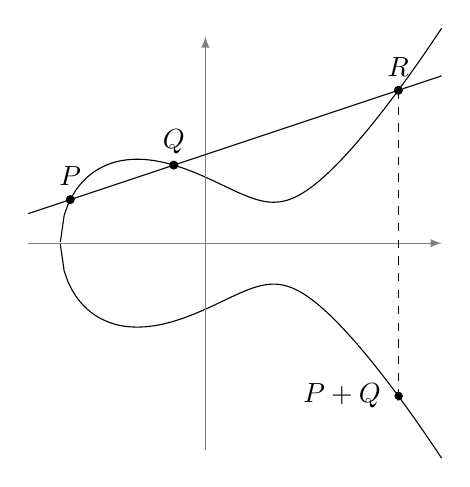
\begin{tikzpicture}[domain=-2.4566:4,samples=100,yscale=3/8,xscale=3/4]
    \draw plot (\x,{sqrt(\x*\x*\x-4*\x+5)});
    \draw plot (\x,{-sqrt(\x*\x*\x-4*\x+5)});

    \draw[thin,gray,-latex] (0,-7) -- (0,7);
    \draw[thin,gray,-latex] (-3,0) -- (4,0);

    \draw (-3,1) -- (4,8/3+3);
    \begin{scope}[every node/.style={draw,circle,inner sep=1pt,fill},cm={1,2/3,0,0,(0,3)}]
      \node at (-2.287980,0) {};
      \node at (-0.535051,0) {};
      \node at (3.267475,0) {};
    \end{scope}
    \begin{scope}[every node/.style={yshift=0.3cm},cm={1,2/3,0,0,(0,3)}]
      \node at (-2.287980,0) {$P$};
      \node at (-0.535051,0) {$Q$};
      \node at (3.267475,0) {$R$};
    \end{scope}

    \draw[dashed] (3.267475,3.267475*2/3+3) -- (3.267475,-3.267475*2/3-3) 
    node[draw,circle,inner sep=1pt,fill] {}
    node[xshift=-0.1cm,anchor=east] {$P+Q$};
  \end{tikzpicture}
  %% 
  \hfill
  %% 
  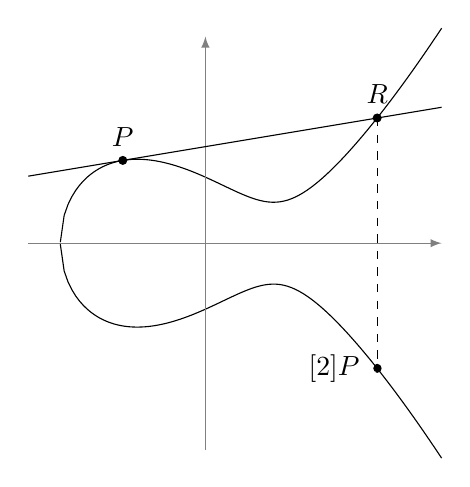
\begin{tikzpicture}[domain=-2.4566:4,samples=100,yscale=3/8,xscale=3/4]
    \draw plot (\x,{sqrt(\x*\x*\x-4*\x+5)});
    \draw plot (\x,{-sqrt(\x*\x*\x-4*\x+5)});

    \draw[thin,gray,-latex] (0,-7) -- (0,7);
    \draw[thin,gray,-latex] (-3,0) -- (4,0);
    
    \def\c{3.269524}
    \def\P{-1.398674}
    \def\R{2.908459}
    \draw (-3,-1+\c) -- (4,4/3+\c);
    \begin{scope}[every node/.style={draw,circle,inner sep=1pt,fill},cm={1,1/3,0,0,(0,3.269524)}]
      \node at (\P,0) {};
      \node at (\R,0) {};
    \end{scope}
    \begin{scope}[every node/.style={yshift=0.3cm},cm={1,1/3,0,0,(0,3.269524)}]
      \node at (\P,0) {$P$};
      \node at (\R,0) {$R$};
    \end{scope}

    \draw[dashed] (\R,\R/3+\c) -- (\R,-\R/3-\c) 
    node[draw,circle,inner sep=1pt,fill] {}
    node[xshift=-0.1cm,anchor=east] {$[2]P$};
  \end{tikzpicture}
  %%
  \hfill
  \strut
  
  \caption{An elliptic curve defined over $ℝ$, and the geometric
    representation of its group law.}
  \label{fig:weierstrass}
\end{figure}

Now, since any elliptic curve is defined by a cubic equation, Bezout's
theorem tells us that any line in $\P^2$ intersects the curve in
exactly three points, taken with multiplicity. %
We define a group law by requiring that three co-linear points sum to
zero. %

\begin{definition}
  Let $E\;:\;y^2=x^3+ax+b$ be an elliptic curve. Let $P_1=(x_1,y_1)$
  and $P_2=(x_2,y_2)$ be two points on $E$ different from the point at
  infinity, then we define a composition law $⊕$ on $E$ as
  follows:
  \begin{itemize}
  \item $P ⊕ \O = \O ⊕ P = P$ for any point $P∈E$;
  \item If $x_1=x_2$ and $y_1=-y_2$, then $P_1⊕P_2 = \O$;
  \item Otherwise set
    \[λ =
      \begin{cases}
        \frac{y_2-y_1}{x_2-x_1} &\text{if $P≠Q$,}\\
        \frac{3x_1+a}{2y_1} &\text{if $P=Q$,}
      \end{cases}
    \]
    then the point $(P_1⊕P_2)=(x_3,y_3)$ is defined by
    \begin{align*}
      x_3 &= λ^2 - x_1 - x_2,\\
      y_3 &= -λx_3 - y_1 + λx_1.
    \end{align*}
  \end{itemize}
\end{definition}

It can be shown that the above law defines an Abelian group, thus we
will simply write $+$ for $⊕$. %
The $n$-th scalar multiple of a point $P$ will be denoted by $[n]P$. %
When $E$ is defined over $k$, the subgroup of its \emph{rational
  points over $k$} is customarily denoted $E(k)$. %
Figure~\ref{fig:weierstrass} shows a graphical depiction of the group
law on an elliptic curve defined over $ℝ$.

We now turn to the group structure of elliptic curves. %
The torsion part is easily characterized.

\begin{proposition}
  Let $E$ be an elliptic curve defined over a field $k$, and let $m≠0$
  be an integer. %
  The $m$-torsion group of $E$, denoted by $E[m]$, has the following
  structure:
  \begin{itemize}
  \item $E[m] ≃ (ℤ/mℤ)^2$ if the characteristic of $k$ does not divide
    $m$;
  \item If $p>0$ is the characteristic of $k$, then 
    \[E[p^i] ≃
      \begin{cases}
        ℤ/p^iℤ & \text{for any $i≥0$,}\\
        \{\O\} & \text{for any $i≥0$.}
      \end{cases}
    \]
  \end{itemize}
\end{proposition}
\begin{proof}
  See~\cite[Coro.~6.4]{silverman:elliptic}. For the characteristic $0$
  case see also next section.
\end{proof}

For curves defined over a field of positive characteristic $p$, the
case $E[p]≃ℤ/pℤ$ is called \emph{ordinary}, while the case
$E[p]≃\{\O\}$ is called \emph{supersingular}.

The free part of the group is much harder to characterize. %
We have some partial results for elliptic curves over number fields.

\begin{theorem}[Mordell-Weil]
  Let $k$ be a number field, the group $E(k)$ is finitely generated.
\end{theorem}

However the exact determination of the rank of $E(k)$ is somewhat
elusive: we have algorithms to compute the rank of most elliptic
curves over number fields; however, an exact formula for such rank is
the object of the
\href{https://en.wikipedia.org/wiki/Birch_and_Swinnerton-Dyer_conjecture}{\it
  Birch and Swinnerton-Dyer conjecture}, one of the
\href{https://en.wikipedia.org/wiki/Millennium_Prize_Problems}{\it
  Clay Millenium Prize Problems}.

\subsection{Maps between elliptic curves}

Finally, we focus on maps between elliptic curves. %
We are mostly interested in maps that preserve both facets of elliptic
curves: as projective varieties, and as groups. %

We first look into invertible algebraic maps, that is linear changes
of coordinates that preserve the Weierstrass form of the equation. %
Because linear maps preserve lines, it is immediate that they also
preserve the group law. %
It is easily verified that the only such maps take the form
\[(x,y) \mapsto (u^2x', u^3y')\] %
for some $u∈\bar{k}$, thus defining an \emph{isomorphism} between the
curve $y^2=x^3+au^4x+bu^6$ and the curve $(y')^2 = (x')^3 + ax' +
b$. %
Isomorphism classes are traditionally encoded by an invariant whose
origins can be tracked back to complex analysis.

\begin{proposition}[$j$-invariant]
  \label{th:j}
  Let $E:y^2=x^3+ax+b$ be an elliptic curve, and define the
  \emph{$j$-invariant} of $E$ as
  \[j(E) = 1728\frac{4a^3}{4a^3+27b^2}.\] %
  Two curves are isomorphic over the algebraic closure $\bar{k}$ if
  and only if they have the same $j$-invariant.
\end{proposition}

Note that if two curves defined over $k$ are isomorphic over
$\bar{k}$, they are so over an extension of $k$ of degree dividing
$6$. %
An isomorphism between two elliptic curves defined over $k$, that is
itself not defined over $k$ is called a \emph{twist}. %
Any curve has a \emph{quadratic twist}, unique up to isomorphism,
obtained by taking $u∉k$ such that $u^2∈k$. %
The two curves of $j$-invariant $0$ and $1728$ also have \emph{cubic},
\emph{sextic} and \emph{quartic twists}.

A surjective group morphism, not necessarily invertible, between two
elliptic curves is called an \emph{isogeny}. %
It turns out that isogenies are algebraic maps as well.

\begin{theorem}
  Let $E,E'$ be two elliptic curves, and let $\phi:E→E$ be a map between
  them. %
  The following conditions are equivalent:
  \begin{enumerate}
  \item $\phi$ is a surjective group morphism,
  \item $\phi$ is a group morphism with finite kernel,
  \item $\phi$ is a non-constant algebraic map of projective varieties
    sending the point at infinity of $E$ onto the point at infinity of
    $E'$.
  \end{enumerate}
\end{theorem}
\begin{proof}
  See\cite[III, Th.~4.8]{silverman:elliptic}.
\end{proof}

Two curves are called \emph{isogenous} if there exists an isogeny
between them. %
We shall see in the next section that this is an equivalence relation.

Isogenies from a curve to itself are called \emph{endomorphisms}. %
The prototypical endomorphism is the multiplication-by-$m$
endomorphism defined by
\[[m]\;:\; P \mapsto [m]P.\] %
Its kernel is exactly the $m$-th torsion subgroup $E[m]$. %
For most elliptic curves, this is the end of the story: the only
endomorphisms are the scalar multiplications. %
We shall however see some non-trivial endomorphisms soon.


\subsection{Elliptic curves over finite fields}

From now on we let $E$ be an elliptic curve defined over a finite
field $k$ with $q$ elements. %
Obviously, the group of $k$-rational points is finite, thus the
algebraic group $E(\bar{k})$ only contains torsion elements, and we
have already characterized precisely the structure of the torsion part
of $E$.

Curves over finite fields always have a non-trivial endomorphism.

\begin{definition}[Frobenius endomorphism]
  Let $E$ be an elliptic curve defined over a field with $q$ elements,
  its \emph{Frobenius endomorphism}, denoted by $π$, is the map that
  sends
  \[(X:Y:Z) \mapsto (X^q:Y^q:Z^q).\]
\end{definition}

\begin{proposition}
  \label{th:frob}
  Let $π$ be the Frobenius endomorphism of $E$. Then:
  \begin{itemize}
  \item $\ker π = \{\O\}$;
  \item $\ker (π-1) = E(k)$.
  \end{itemize}
\end{proposition}

\begin{corollary}[Hasse's theorem]
  Let $E$ be an elliptic curve defined over a finite field $k$ with $q$
  elements, then
  \[|\#E(k) - q - 1| ≤ 2\sqrt{q}.\]
\end{corollary}
\begin{proof}
  See\cite[V, Th.~1.1]{silverman:elliptic}.
\end{proof}

It turns out that the cardinality of $E$ over its \emph{base field}
$k$ determines its cardinality over any finite extension of it. %
This is a special case of a special case of the famous \emph{Weil's
  conjectures}, proven by Weil himself in 1949 for Abelian varieties,
and more generally by Deligne in 1973.

\begin{definition}
  Let $V$ be a projective variety defined over a finite field $\F_q$,
  its \emph{zeta function} is the power series
  \[Z(V/\F_q; T) = \exp\left(\sum_{n=1}^∞\#V(\F_{q^n})\frac{T^n}{n}\right).\]
\end{definition}

\begin{theorem}
  \label{th:weil}
  Let $E$ be an elliptic curve defined over a finite field
  $\F_q$, and let $\#E(\F_q)=q+1-a$. Then
  \[Z(E/\F_q;T) = \frac{1-aT+qT^2}{(1-T)(1-qT)}.\]
\end{theorem}
\begin{proof}
  See~\cite[V, Th.~2.4]{silverman:elliptic}.
\end{proof}

We conclude with a theorem that links the isogenies between two
elliptic curves with their Frobenius endomorphisms.

\begin{theorem}[Sato-Tate]
  Two elliptic curves $E,E'$ defined over a finite field $k$ are
  isogenous over $k$ if and only if $\#E(k)=\#E'(k)$.
\end{theorem}


\subsection{Application: Diffie-Hellman key exhange}
\label{sec:appl-diff-hellm}

Elliptic curves are largely present in modern technology thanks to
their applications in cryptography. %
The simplest of these application is the \emph{Diffie-Hellman key
  exchange}, a cryptographic protocol by which two parties
communicating over a public channel can agree on a common secret
string unknown to any other party listening on the same channel.

The original protocol was invented in the 1970s by Whitfield Diffie
and Martin Hellman~\cite{dh}, and constitutes the first practical
example of \emph{public key cryptography}. %
The two communicating parties are customarily called \emph{Alice} and
\emph{Bob}, and the listening third party is represented by the
character \emph{Eve} (for \emph{eavesdropper}). %
To set up the protocol, Alice and Bob agree on a set of public
parameters:
\begin{itemize}
\item A \emph{large enough} prime number $p$, such that $p-1$ has a
  \emph{large enough} prime factor;
\item A multiplicative generator $g∈ℤ/pℤ$.
\end{itemize}

Then, Alice and Bob perform the following steps:
\begin{enumerate}
\item Each chooses a \emph{secret} integer in the interval $]0,p-1[$;
  call $a$ \emph{Alice's secret} and $b$ \emph{Bob's secret}.
\item They respectively compute $A=g^a$ and $B=g^b$.
\item They exchange $A$ and $B$ over the public channel.
\item They respectively compute the \emph{shared secret}
  $B^a=A^b=g^{ab}$.
\end{enumerate}

The protocol can be easily generalized by replacing the multiplicative
group $(ℤ/pℤ)^×$ with any other cyclic group $G=〈g〉$. %
From Eve's point of view, she is given the knowledge of the group $G$,
the generator $g$, and Alice's and Bob's public data $A,B∈G$; her goal
is to recover the shared secret $g^{ab}$. %
This is mathematically possible, but not necessarily \emph{easy} from
a computational point of view.

\begin{definition}[Discrete logarithm]
  Let $G$ be a cyclic group generated by an element $g$. For any
  element $A∈G$, we define the \emph{discrete logarithm of $A$ in base
    $g$}, denoted $\log_g(A)$, as the unique integer in the interval
  $[0,\#G[$ such that
  \[g^{\log_g(A)} = A.\]
\end{definition}

It is evident that if Eve can compute discrete logarithms in $G$, then
she can compute the shared secret; the converse is not true in
general, but it is widely believed to be. %
Thus, the strength of the Diffie-Hellman protocol is entirely
dependent on the \emph{hardness} of the \emph{discrete logarithm
  problem} in the group $G$.

We know algorithms to compute discrete logarithms in a \emph{generic}
group $G$ that require $O(\sqrt{q})$ computational steps
(see~\cite{joux2009algorithmic}), where $q$ is the largest prime
divisor of $\#G$; we also know that these algorithms are \emph{optimal
  for abstract cyclic groups}. %
For this reason, $G$ is usually chosen so that the largest prime
divisor $q$ has size at least $\log_2 q ≈ 256$. %
However, the proof of optimally does not exclude the existence of
better algorithms for \emph{specific} groups $G$. %
And indeed, algorithms of complexity better than $O(\sqrt{\#G})$ are
known for the case $G=(ℤ/pℤ)^×$~\cite{joux2009algorithmic}, thus
requiring parameter of considerably larger size to guarantee
cryptographic strength.

On the contrary, no algorithms better than the generic ones are known
when $G$ is a subgroup of $E(k)$, where $E$ is an elliptic curve
defined over a finite field $k$. %
This has led Miller~\cite{miller86} and Koblitz~\cite{koblitz87} to
suggest, in the 1980s, to replace $(ℤ/pℤ)^×$ in the Diffie-Helman
protocol by the group of rational points of an elliptic curve of
(almost) prime order over a finite field. %
The resulting protocol is summarized in Figure~\ref{fig:dh}.

\begin{figure}
  \centering
  \begin{tabular}{l *{2}{p{0.25\textwidth}<{\centering}}}
    \hline
    Public parameters & \multicolumn{2}{l}{Finite field $\F_p$, with $\log_2p≈256$,}\\
                      & \multicolumn{2}{l}{Elliptic curve $E/\F_p$, such that $\#E(\F_p)$ is prime,}\\
                      & \multicolumn{2}{l}{A generator $P$ of $E(\F_p)$.}\\
    \hline
                      & {\bf Alice} & {\bf Bob}\\
    \hline
    Pick random secret & $0<a<\#E(\F_p)$ & $0<b<\#E(\F_p)$\\
    Compute public data & $A = [a]P$ & $B = [b]P$\\
    Exchange data &  \hfill $A \longrightarrow$ & $\longleftarrow B$ \hfill\strut \\
    Compute shared secret & $S = [a]B$ & $S = [b]A$
  \end{tabular}
  
  \caption{The Diffie-Hellman protocol over elliptic curves}
  \label{fig:dh}
\end{figure}


\subsection{Application: Elliptic curve factoring method}

A second popular use of elliptic curves in technology is for factoring
large integers, a problem that also occurs frequently in cryptography.

The earliest method for factoring integers was already known to the
ancient Greeks: the \emph{sieve of Eratosthenes} finds all primes up
to a given bound by crossing composite numbers out in a table. %
Applying the Eratosthenes' sieve up to $\sqrt{N}$ finds all prime
factors of a composite number $N$. %
Examples of modern algorithms used for factoring are Pollard's
\emph{Rho algorithm} and Coppersmith's \emph{Number Field Sieve
  (NFS)}.

In the 1980s H. Lenstra~\cite{lenstra87} introduced an algorithm for
factoring that has become known as the \emph{Elliptic Curve Method
  (ECM)}. %
Its complexity is between Pollard's and Coppersmith's algorithms in
terms of number of operations; at the same time it only requires a
constant amount of memory, and is very easy to parallelize. %
For these reasons, ECM is typically used to factor integers having
medium sized prime factors.

From now on we suppose that $N=pq$ is an integer whose factorization
we wish to compute, where $p$ and $q$ are distinct primes. %
Without loss of generality, we can suppose that $p<q$.

Lenstra's idea has its roots in an earlier method for factoring
special integers, also due to Pollard. %
Pollard's \emph{$(p-1)$ factoring method} is especially suited for
integers $N=pq$ such that $p-1$ only has \emph{small} prime factors. %
It is based on the isomorphism
\begin{align*}
  \rho : ℤ/Nℤ &\to ℤ/pℤ × ℤ/qℤ,\\
  x &\mapsto (x \bmod p, x \bmod q)
\end{align*}
given by the Chinese remainder theorem. %
The algorithm is detailed in Figure~\ref{fig:p-1}. %
It works by guessing a multiple $e$ of $p-1$, then taking a random
element $x∈(ℤ/Nℤ)^×$, to deduce a random element $y$ in
$〈1〉⊕(ℤ/qℤ)^×$. If the guessed exponent $e$ was correct, and if
$y≠1$, the gcd of $y-1$ with $N$ yields a non-trivial factor. %

\begin{figure}
  \begin{subfigure}{0.45\textwidth}
    \begin{algorithmic}[1]
      \REQUIRE An integer $N=pq$,\\
      a bound $B$ on the largest prime factor of $p-1$;
      \ENSURE $(p,q)$ or FAIL.
      \STATE Set $e = \prod_{r \text{ prime } < B} r^{\lfloor\log_r\sqrt{N}\rfloor}$;
      \STATE Pick a random $1 < x < N$;
      \STATE Compute $y = x^e \mod N$;
      \STATE Compute $q' = \gcd(y-1, N)$;
      \IF {$q' ≠ 1,N$}
      \RETURN $N/q', q'$;
      \ELSE
      \RETURN FAIL.
      \ENDIF
    \end{algorithmic}
    
    \caption{Pollard's $(p-1)$ algorithm}
    \label{fig:p-1}
  \end{subfigure}
  %% 
  \hfill
  %% 
  \begin{subfigure}{0.45\textwidth}
    \begin{algorithmic}[1]
      \REQUIRE An integer $N=pq$, a bound $B$;
      \ENSURE $(p,q)$ or FAIL.
      \STATE Pick random integers $a,X,Y$ in $[0,N[$;
      \STATE Compute $b = Y^2 - X^3 - aX \mod N$;
      \STATE Define the elliptic curve $E \;:\; y^2 = x^3 - ax - b$.
      \STATE Define the point $P=(X:Y:1) ∈ E(ℤ/Nℤ)$.
      \STATE Set $e = \prod_{r \text{ prime } < B} r^{\lfloor\log_r\sqrt{N}\rfloor}$;
      \STATE Compute $Q = [e]P = (X':Y':Z')$;
      \STATE Compute $q' = \gcd(Z', N)$;
      \IF {$q' ≠ 1,N$}
      \RETURN $N/q', q'$;
      \ELSE
      \RETURN FAIL.
      \ENDIF
    \end{algorithmic}
    
    \caption{Lenstra's ECM algorithm}
    \label{fig:ecm}
  \end{subfigure}
  \caption{The $(p-1)$ and ECM factorization algorithms}
\end{figure}

The $p-1$ method is very effective when the bound $B$ is small, but
its complexity grows exponentially with $B$. %
For this reason it is only usable when $p-1$ has small prime factors,
a constraint that is very unlikely to be satisfied by random primes.

Lenstra's ECM algorithm is a straightforward generalization of the
$p-1$ method, where the multiplicative groups $(ℤ/pℤ)^×$ and
$(ℤ/qℤ)^×$ are replaced by the groups of points $E(\F_p)$ and
$E(\F_q)$ of an elliptic curve defined over $ℚ$. %
Now, the requirement is that $\#E(\F_p)$ only has small prime
factors. %
This condition is also extremely rare, but now we have the freedom to
try the method many times by changing the elliptic curve. %

The algorithm is summarized in Figure~\ref{fig:ecm}. %
It features two remarkable subtleties. %
First, it would feel natural to pick a random elliptic curve
$E:y^2=x^3+ax+b$ by picking random $a$ and $b$, however taking a point
on such curve would then require computing a square root modulo $N$, a
problem that is known to be has hard as factoring $N$. %
For this reason, the algorithm starts by taking a random point, and
then deduces the equation of $E$ from it. %
Secondly, all computations on coordinates happen in the projective
plane over $ℤ/Nℤ$; however, properly speaking, projective space cannot
be defined over non-integral rings. %
Implicitly, $E(ℤ/Nℤ)$ is defined as the product group
$E(\F_p)⊕E(F_q)$, and any attempt at inverting a non-invertible in
$ℤ/Nℤ$ will result in a factorization of $N$.

\subsection*{Exercices}

\begin{exercice}
  Prove Proposition~\ref{th:j}.
\end{exercice}

\begin{exercice}
  Determine all the possible automorphisms of elliptic curves.
\end{exercice}

\begin{exercice}
  Prove Proposition~\ref{th:frob}.
\end{exercice}

\begin{exercice}
  Using Proposition~\ref{th:weil}, devise an algorithm to effectively
  compute $\#E(\F_{q^n})$ given $\#E(\F_q)$.
\end{exercice}

\begin{exercice}
  Implement the ECDH key exchange in the language of your choice.
\end{exercice}

\begin{exercice}[Polig-Hellman algorithm]
  Let $G$ be a cyclic group of order $N=pq$, generated by an element
  $g$. %
  Show how to solve discrete logarithms in $G$ by computing two
  separate discrete logarithms in the subgroups $〈g^p〉$ and $〈g^q〉$.
\end{exercice}

\begin{exercice}
  Implement the ECM factorization method in the language of your
  choice.
\end{exercice}

%%%%%%%%%%%%%%%%%%%%%%%%%%%%%%%%%%%%%%%%%%%%%%%%%%%%%%

\clearpage

\section{Isogenies and applications}

\subsection{Elliptic curves over $ℂ$}

\begin{definition}[Complex lattice]
  A complex lattice $Λ$ is a discrete subgroup of $ℂ$ that contains an
  $ℝ$-basis.
\end{definition}

Explicitly, a complex lattice is generated by a \emph{basis}
$(ω_1,ω_2)$, such that $ω_1≠λω_2$ for any $λ∈ℝ$, as
\[Λ = ω_1ℤ + ω_2ℤ.\] %
Up to exchanging $ω_1$ and $ω_2$, we can assume that $\im(ω_1/ω_2)>0$;
we then say that the basis has \emph{positive orientation}. %
A positively oriented basis is obviously not unique, though.

\begin{proposition}
  \label{th:basis-change}
  Let $Λ$ be a complex lattice, and let $(ω_1,ω_2)$ be a positively
  oriented basis, then any other positively oriented basis
  $(ω_1',ω_2')$ is of the form
  \begin{align*}
    ω_1' &= aω_1 + bω_2,\\
    ω_1' &= cω_1 + dω_2,
  \end{align*}
  for some matrix
  $\left(\begin{smallmatrix}a&b\\c&d\end{smallmatrix}\right)∈\SL_2(ℤ)$.
\end{proposition}
\begin{proof}
  See~\cite[I, Lem.~2.4]{silverman:advanced}.
\end{proof}

\begin{definition}[Complex tours]
  Let $Λ$ be a complex lattice, the quotient $ℂ/Λ$ is called a
  \emph{complex torus}.
\end{definition}

\begin{figure}
  \centering
  \begin{tikzpicture}[scale=2]
    \axes{-1}{3.5}{-0.5}{3}

    \begin{scope}[/lattice={1}{0.2}{0.4}{0.7}]
      \draw[fill,black!10] (0,0) -- (1,0) -- (1,1) -- (0,1) -- (0,0);
      \node at (0.5,0.5) {$ℂ/Λ$};
      \node at (0.9,-0.1) {$ω_2$};
      \node at (-0.1,0.9) {$ω_1$};

      \lattice{-3}{4}
    \end{scope}  
  \end{tikzpicture}

  \caption{A complex lattice (black dots) and its associated complex
    torus (grayed \emph{fundamental domain}).}
  \label{fig:lattice}
\end{figure}

A convex set of class representatives of $ℂ/Λ$ is called a
\emph{fundamental parallelogram}. %
Figure~\ref{fig:lattice} shows a complex lattice generated by a
(positively oriented) basis $(ω_1,ω_2)$, together with a fundamental
parallelogram for $ℂ/(ω_1,ω_2)$. %
The additive group structure of $ℂ$ carries over to $ℂ/Λ$, and can be
graphically represented as operations on points inside a fundamental
parallelogram. %
This is illustrated in Figure~\ref{fig:lattice-arith}.

\begin{figure}
  \centering
  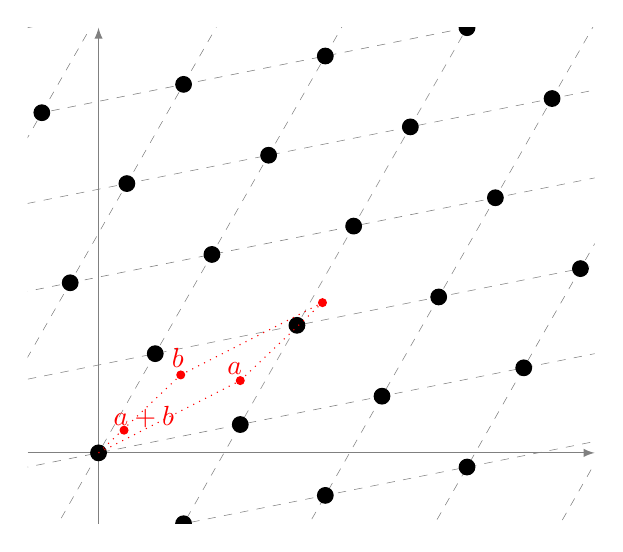
\begin{tikzpicture}[scale=1.8]
    \axes{-0.5}{3.5}{-0.5}{3}

    \begin{scope}[/lattice={1}{0.2}{0.4}{0.7}]
      \lattice{-3}{4}

      \node[red] at (0.7,0.65) {$a$}; 
      \node[draw,circle,inner sep=1pt,fill,red] at (0.8,0.5) {};
      \node[red] at (0.2,0.9) {$b$}; 
      \node[draw,circle,inner sep=1pt,fill,red] at (0.3,0.7) {};
      
      \node[draw,circle,inner sep=1pt,fill,red] at (1.1,1.2) {};

      \draw[red,thin,dotted] (0,0) -- (0.8,0.5) -- (1.1,1.2)
      (0,0) -- (0.3,0.7) -- (1.1,1.2);          

      \node[red] at (0.2,0.3) {$a+b$}; 
      \node[draw,circle,inner sep=1pt,fill,red] at (0.1,0.2) {};
    \end{scope}  
  \end{tikzpicture}
  %%
  \hfill
  %%
  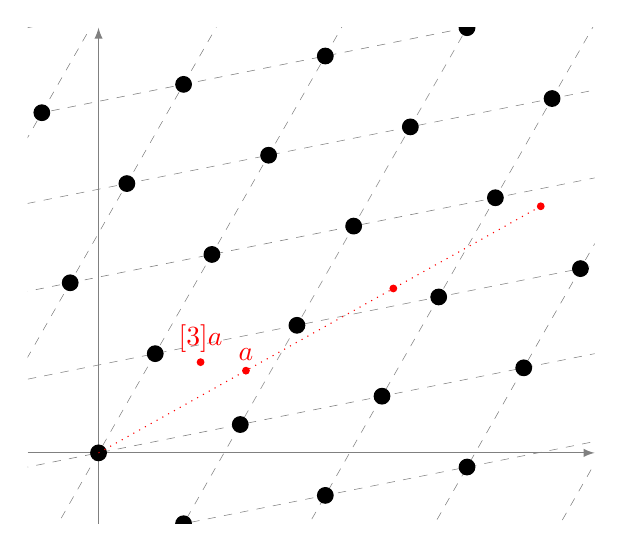
\begin{tikzpicture}[scale=1.8]
    \axes{-0.5}{3.5}{-0.5}{3}

    \begin{scope}[/lattice={1}{0.2}{0.4}{0.7}]
      \lattice{-3}{4}
      
      \node[red,yshift=0.2cm] at (0.8,0.6) {$a$}; 
      \draw[red] (0.8,0.6) node[fill,circle,inner sep=1pt] {};

      \draw[red,dotted] (0,0) -- (1.6,1.2) node[fill,circle,inner sep=1pt] {} 
      -- (2.4,1.8) node[fill,circle,inner sep=1pt] {};

      \node[red,yshift=0.3cm] at (0.4,0.8) {$[3]a$}; 
      \draw[red] (0.4,0.8) node[fill,circle,inner sep=1pt] {};
    \end{scope}
  \end{tikzpicture}
  \caption{Addition (left) and scalar multiplication (right) of points
    in a complex torus $ℂ/Λ$.}
  \label{fig:lattice-arith}
\end{figure}

\begin{definition}[Homothetic lattices]
  Two complex lattices $Λ$ and $Λ'$ are said to be \emph{homothetic}
  if there is a complex number $α∈ℂ^×$ such that $Λ=αΛ'$.
\end{definition}

Geometrically, applying a homothety to a lattice corresponds to zooms
and rotations around the origin. %
We are only interested in complex tori up to homothety; to classify
them, we introduce the \emph{Eisenstein series of weight $2k$},
defined as
\[G_{2k}(Λ) = \sum_{ω∈Λ\setminus\{0\}}ω^{-2k}.\]
It is customary to set
\[g_2(Λ) = 60G_4(Λ), \quad g_3(Λ) = 140G_6(Λ);\] %
when $Λ$ is clear from the context, we simply write $g_2$ and $g_3$.

\begin{theorem}[Modular $j$-invariant]
  The \emph{modular $j$-invariant} is the function on complex lattices
  defined by
  \[j(Λ) = 1728 \frac{g_2(Λ)^3}{g_2(Λ)^3 - 27g_3(Λ)^2}.\] %
  Two lattices are homothetic if and only if they have the same
  modular $j$-invariant.
\end{theorem}
\begin{proof}
  See~\cite[I, Th.~4.1]{silverman:advanced}.
\end{proof}

It is no chance that the invariants classifying elliptic curves and
complex tori look very similar. %
Indeed, we can prove that the two are in one-to-one correspondence.

\begin{definition}[Weierstrass $℘$ function]
  Let $Λ$ be a complex lattice, the \emph{Weierstrass $℘$ function}
  associated to $Λ$ is the series
  \[℘(z;Λ) = \frac{1}{z^2} + \sum_{ω∈Λ\setminus\{0\}} \left(\frac{1}{(z-ω)^2} - \frac{1}{ω^2}\right).\]
\end{definition}

\begin{theorem}
  The Weierestrass function $℘(z;Λ)$ has the following properties:
  \begin{enumerate}
  \item It is an \emph{elliptic function} for $Λ$, i.e.
    $℘(z) = ℘(z+ω)$ for all $z∈ℂ$ and $ω∈Λ$.
  \item Its Laurent series around $z=0$ is
    \[℘(z) = \frac{1}{z^2} + \sum_{k=1}^∞(2k+1)G_{2k+2}z^{2k}.\]
  \item It satisfies the differential equation
    \[℘'(z)^2 = 4℘(z)^3 - g_2℘(z) - g_3\]
    for all $z∉Λ$.
  \item The curve
    \[E\;:\;y^2=4x^3 - g_2x - g_3\]
    is an elliptic curve over $ℂ$. The map
    \begin{align*}
      ℂ/Λ &\to E(ℂ),\\
      0 &\mapsto (0:1:0),\\
      z &\mapsto (℘(z):℘'(z):1)
    \end{align*}
    is an isomorphism of Riemann surfaces and a group morphism.
  \end{enumerate}
\end{theorem}
\begin{proof}
  See~\cite[VI, Th.~3.1, Th.~3.5, Prop.~3.6]{silverman:elliptic}.
\end{proof}

By comparing the two definitions for the $j$-invariants, we see that
$j(Λ)=j(E)$. %
So, for any homotety class of complex tori, we have a corresponding
isomorphism class of elliptic curves. %
The converse is also true.

\begin{theorem}[Uniformization theorem]
  Let $a,b∈ℂ$ be such that $4a^3+27b^2≠0$, then there is a unique
  complex lattice $Λ$ such that $g_2(Λ) = -4a$ and $g_3(Λ) = -4b$.
\end{theorem}
\begin{proof}
  See~\cite[I, Coro.~4.3]{silverman:advanced}.
\end{proof}

Using the correspondence between elliptic curves and complex tori, we
now have a new perspective on their group structure. %
Looking at complex tori, it becomes immediately evident why the
torsion part has rank $2$, i.e. why $E[m]≃(ℤ/mℤ)^2$. %
This is illustrated in Figure~\ref{fig:torsion}; in the picture wee
see two lattices $Λ$ and $Λ'$, generated respectively by the black and
the red dots. %
The multiplication-by-$m$ map corresponds then to
\begin{align*}
  [m] : ℂ/Λ &\to ℂ/Λ',\\
  z &\mapsto z \bmod Λ';
\end{align*}
and we verify that it is and endomorphism because $Λ$ and $Λ'$ are
homothetic.

\begin{figure}

  \begin{subfigure}{.45\textwidth}
    \centering
    
    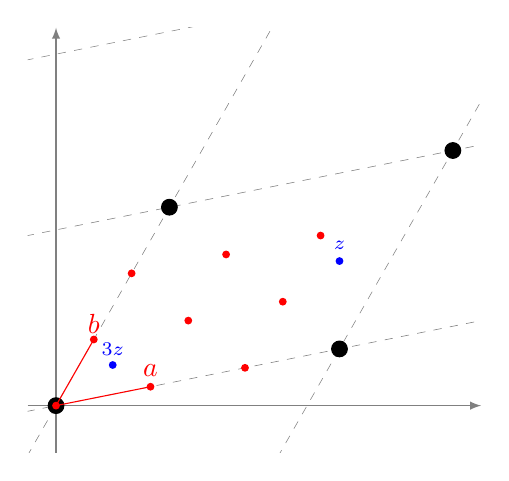
\begin{tikzpicture}[scale=1.2]
      \axes{-0.3}{4.5}{-0.5}{4};

      \begin{scope}[/lattice={3}{0.6}{1.2}{2.1}]
        \lattice{-1}{2}

        \foreach \i in {0,...,2} {
          \foreach \j in {0,...,2} {
            \draw[red] (\i/3,\j/3) node[fill,circle,inner sep=1pt] {};
          }
        }
        \draw[red] (0,0) -- (1/3,0) node[yshift=0.2cm] {$a$};
        \draw[red] (0,0) -- (0,1/3) node[yshift=0.2cm] {$b$};

        \draw[blue] (0.8,0.5) node[fill,circle,inner sep=1pt] {}
        node[yshift=0.2cm] {\scriptsize $z$}
        (2/15,1/6) node[fill,circle,inner sep=1pt] {}
        node[yshift=0.2cm] {\scriptsize $3z$};
      \end{scope}
    \end{tikzpicture}  
    \caption{$3$-torsion group on a complex torus (red
      points), with two generators $a$ and $b$, and action of the
      multiplication-by-$3$ map (blue dots).}
    \label{fig:torsion}
  \end{subfigure}
  %%
  \hfill
  %%
  \begin{subfigure}{.45\textwidth}
    \centering
    \begin{tikzpicture}[scale=1.2]
      \axes{-0.3}{4.5}{-0.5}{4};
      
      \begin{scope}[/lattice={3}{0.6}{1.2}{2.1}]
        \lattice{-1}{2}

        \draw[red] (0,0) -- (1/3,0) node[yshift=0.3cm] {$a$};
        \draw[green] (0,0) -- (0,1/3) node[fill,circle,inner sep=1pt] {}
        node[yshift=0.3cm] {$b$};

        \draw[blue] (0.8,0.5) node[fill,circle,inner sep=1pt] {}
        node[yshift=0.3cm] {$z$};
      \end{scope}
      
      \begin{scope}[/lattice={1}{0.2}{1.2}{2.1}]
        \begin{scope}[opacity=0.5,red]
          \lattice[1pt]{-3}{5}
        \end{scope}

        \draw[blue] (0.4,0.5) node[fill,circle,inner sep=1pt] {}
        node[yshift=0.3cm] {$ϕ(z)$};
      \end{scope}
    \end{tikzpicture}
    
    \caption{Isogeny from $ℂ/Λ$ (black dots) to $ℂ/Λ'$ (red dots)
      defined by $ϕ(z)=z \bmod Λ'$. The kernel of $ϕ$ is contained
      in $(ℂ/Λ)[3]$ and is generated by $a$. The kernel of the dual
      isogeny $\hat{ϕ}$ is generated by the vector $b$ in $Λ'$.}
    \label{fig:isogeny}
  \end{subfigure}
  
  \caption{Maps between complex tori.}
\end{figure}

Within this new perspective, isogenies are a mild generalization of
scalar multiplications. %
Whenever two lattices $Λ,Λ'$ verify $αΛ⊂Λ'$, there is a well defined
map
\begin{align*}
   ϕ_α : ℂ/Λ &\to ℂ/Λ',\\
  z &\mapsto αz \bmod Λ'
\end{align*}
that is holomorphic and also a group morphism. %
One example of such maps is given in Figure~\ref{fig:torsion}: there,
$α=1$ and the red lattice strictly contains the black one; the map is
simply defined as reduction modulo $Λ'$. %
It turns out that these maps are exactly the isogenies of the
corresponding elliptic curves.

\begin{theorem}
  Let $E,E'$ be elliptic curves over $ℂ$, with corresponding lattices
  $Λ,Λ'$. %
  There is a bijection between the group of isogenies from $E$ to $E'$
  and the group of maps $ϕ_α$ for all $α$ such that $Λ⊂αΛ'$.
\end{theorem}
\begin{proof}
  See~\cite[VI, Th.~4.1]{silverman:elliptic}.
\end{proof}

Looking again at Figure~\ref{fig:torsion}, we see that there is a
second isogeny $\hat{ϕ}$ from $Λ'$ to $Λ/3$, whose kernel is generated
by $b∈Λ'$. %
The composition $\hat{ϕ}∘ϕ$ is an endomorphism of $ℂ/Λ$, up to the
homothety sending $Λ/3$ to $Λ$, and we verify that it corresponds to
the multiplication-by-$3$ map. %
In this example, the kernels of both $ϕ$ and $\hat{ϕ}$ contain $3$
elements, and we say that $ϕ$ and $\hat{ϕ}$ have \emph{degree} $3$. %
Although not immediately evident from the picture, this same
construction can be applied to any isogeny. %
The isogeny $\hat{ϕ}$ is called the \emph{dual} of $ϕ$. %
Dual isogenies exist not only in characteristic $0$, but for any base
field. %

We finish this section by summarizing the most important algebraic
properties of isogenies; we start with a technical definition.

\begin{definition}[Degree]
  Let $ϕ:E\to E'$ be an isogeny defined over a field $k$, and let
  $k(E),k(E')$ be the function fields of $E,E'$. %
  By composing $\phi$ with the functions of $k(E')$, we obtain a
  subfield of $k(E)$ that we denote by $ϕ^\ast(k(E'))$.

  \begin{enumerate}
  \item The \emph{degree} of $ϕ$ is defined as
    $\deg ϕ = [k(E):ϕ^\ast(k(E'))]$; it is always finite.
  \item $ϕ$ is said to be \emph{separable}, \emph{inseparable}, or
    \emph{purely inseparable} if the extension of function fields is.
  \item If $ϕ$ is separable, then $\deg ϕ = \#\ker ϕ$.
  \item If $ϕ$ is purely inseparable, then $\deg ϕ$ is a power of the
    characteristic of $k$.
  \item Any isogeny can be decomposed as a product of a separable and
    a purely inseparable isogeny.
  \end{enumerate}
\end{definition}
\begin{proof}
  See~\cite[II, Th.~2.4]{silverman:elliptic}.
\end{proof}

In practice, most of the time we will be considering separable
isogenies, and we can take $\deg ϕ = \#\ker ϕ$ as the definition of
the degree. %
Notice that in this case $\deg ϕ$ is the size of any fiber of $ϕ$.

\begin{theorem}[Dual isogeny]
  Let $ϕ:E\to E'$ be an isogeny of degree $m$. %
  There is a unique isogeny $\hat{ϕ}:E'\to E$ such that
  \[\hat{ϕ}∘ϕ = [m]_E, \quad ϕ∘\hat{ϕ} = [m]_{E'}.\] %
  $\hat{ϕ}$ is called the \emph{dual isogeny of $ϕ$}; it has the
  following properties:
  
  \begin{enumerate}
  \item $\hat{ϕ}$ is defined over $k$ if and only if $ϕ$ is;
  \item $\widehat{ψ∘ϕ} = \hat{ϕ}∘\hat{ψ}$ for any isogeny $ψ:E'\to E''$;
  \item $\widehat{ψ+ϕ} = \hat{ψ} + \hat{ϕ}$ for any isogeny $ψ:E\to E'$;
  \item $\deg ϕ = \deg\hat{ϕ}$;
  \item $\hat{\hat{ϕ}} = ϕ$.
  \end{enumerate}
\end{theorem}


\subsection{The endomorphism ring}

We have already defined an endomorphism as an isogeny from a curve to
itself. %
If we add the multiplication-by-$0$, the set of all endomorphisms of
$E$ form a ring under the operations of addition and composition,
denoted by $\End(E)$. %

We have already seen that the multiplication-by-$m$ is a different
endomorphism for any integer $m$, thus $ℤ⊂\End(E)$. %
For the case of finite fields, we have also learned about the
Frobenius endomorphism $π$; so certainly $ℤ[π]⊂\End(E)$ in this
case. %
We shall now give a complete characterization of the endomorphism ring
for any field.

\begin{definition}[Order]
  Let $K$ be a finitely generated $ℚ$-algebra. %
  An \emph{order} $\O⊂K$ is a subring of $K$ that is a finitely
  generated $ℤ$-module of maximal dimension.
\end{definition}

The prototypical example of order is the ring of integers $\O_K$ of a
number field $K$, i.e., the ring of all elements of $K$ such that
their monic minimal polynomial has coefficients in $ℤ$. %
It turns out that $\O_K$ is the \emph{maximal order} of $K$, i.e., it
contains any other order of $K$.

\begin{definition}[Quaternion algebra]
  A \emph{quaternion algebra} is an algebra of the form
  \[K = ℚ + αℚ + βℚ + αβℚ,\]
  where the generators satisfy the relations
  \[α^2,β^2∈ℚ, \quad α^2<0, \quad β^2 < 0, \quad βα=-αβ.\]
\end{definition}

\begin{theorem}[Deuring]
  Let $E$ be an elliptic curve defined over a field $k$ of
  characteristic $p$. %
  The ring $\End(E)$ is isomorphic to one of the following:
  \begin{itemize}
  \item $ℤ$, only if $p=0$;
  \item An order in a quadratic imaginary field (a number field of the
    form $ℚ[\sqrt{-D}]$ for some $D>0$); in this case we say that $E$
    has \emph{complex multiplication};
  \item Only if $p>0$, a maximal order in the quaternion algebra
    ramified at $p$ and $∞$; in this case we say that $E$ is
    \emph{supersingular}.
  \end{itemize}
\end{theorem}
\begin{proof}
  See~\cite[III, Coro.~9.4]{silverman:elliptic}
  and~\cite{belding08-thesis}.
\end{proof}

In positive characteristic, a curve that is not supersingular is
called \emph{ordinary}; it necessarily has complex multiplication. %
We focus again on the finite field case; we have already seen that
$Ζ[π]⊂\End(E)$. %
Now, Hasse's theorem can be made more precise as follows.

\begin{theorem}
  Let $E$ be an elliptic curve defined over a finite field. %
  Its Frobenius endomorphism $π$ satisfies a quadratic equation
  \[π^2 - tπ + q = 0,\]
  for some $|t|≤2\sqrt{q}$.
\end{theorem}
\begin{proof}
  See~\cite[V, Th.~2.3.1]{silverman:elliptic}.
\end{proof}

The coefficient $t$ in the equation is called the \emph{trace} of
$π$. %
By replacing $π=1$ in the equation, we immediately obtain the
cardinality of $E$ as $\#E = q+1-t$. %
Now, if we let $D_π=t^2-4q<0$, we verify that $π∈ℚ[\sqrt{D_π}]$; so,
at least in the ordinary case, we can affirm that
\[ℤ[π] ⊂ \End(E) ⊂ \O_K,\] %
where $K=ℚ[\sqrt{D_π}]$ is called the \emph{endomorphism algebra} of
$E$. %
The structure of the orders of $K$ is very simple in this case.

\begin{proposition}
  Let $K$ be a quadratic number field, and let $\O_K$ be its ring of
  integers. %
  Any order $\O⊂K$ can be written as $\O=ℤ+f\O_K$ for an integer $f$,
  called the \emph{conductor} of $\O$. %
  If $d_K$ is the \emph{discriminant} of $K$, the discriminant of $\O$
  is $f^2d_K$.

  If $\O,\O'$ are two orders of discriminants $f,f'$, then $\O⊂\O'$ if
  and only if $f'|f$.
\end{proposition}

In our case, we can write $D_π=f^2d_K$, with $d_K$
squarefree. % TODO: check this!
Then, any order $ℤ[π] ⊂ \O ⊂ \O_K$ has conductor dividing $f$.

\subsection*{Application: point counting}

Before going more in depth into the study of the endomorphism ring,
let us pause for a while on a simpler problem. %
Hasse's theorem relates the cardinality of a curve defined over a
finite field with the trace of its Frobenius endomorphism. %
However, it does not give us an algorithm to compute either.

The first efficient algorithm to compute the trace of $π$ was proposed
by Schoof in the 1980s~\cite{schoof85}. %
The idea is very simple: compute the value of $t_π\bmod ℓ$ for many
small primes $ℓ$, and then reconstruct the trace using the Chinese
remainder theorem. %
To compute $t_π\bmod ℓ$, Schoof's algorithm formally constructs the
group $E[ℓ]$, takes a generic point $P∈E[\ell]$, and then runs a
search for the integer $t$ such that
\[π([t]P) = [q]P + π^2(P).\]

The algorithm runs in time polynomial in $\log\#E(k)$, however it is
quite slow in practice. %
Among the major advances that have enabled the use of elliptic curves
in cryptography are the optimizations of Schoof's algorithm due to
Atkin and Elkies~\cite{schoof95}. %
Both improvements use a better understanding of the action of $π$ on
$E[ℓ]$. %
Assume that $ℓ$ is different from the characteristic, we have already
seen that $E[ℓ]$ is a group of rank two. %
Hence, $π$ acts on $E[ℓ]$ like a matrix $M$ in $\GL_2(ℤ/ℓℤ)$, and its
characteristic polynomial is exactly
\[χ(X) = X^2 - t_πX + q \mod \ell.\] %
Now we have three possibilities:
\begin{itemize}
\item $χ$ splits modulo $ℓ$, as $χ(X) = (X-λ)(X-μ)$, with $λ≠μ$; we call
  this the \emph{Elkies case}.
\item $χ$ does not split modulo ℓ; we call this the \emph{Atkin case};
\item $χ$ is a square modulo $ℓ$.
\end{itemize}

The SEA algorithm, treats each of these cases in a slightly different
way; for simplicity, we will only sketch the Elkies case. %
In this case, there exists a basis $〈P,Q〉$ for $E[ℓ]$ onto which $π$
acts as a matrix
$M=\left(\begin{smallmatrix}λ&0\\0&μ\end{smallmatrix}\right)$. %
Each of the two eigenspaces of $M$ is the kernel of an isogeny of
degree $ℓ$ from $E$ to another curve $E'$. %
If we can determine $E'$ corresponding to, e.g., $〈P〉$, then we can
compute the isogeny $ϕ:E\to E'$, and use it to formally represent the
point $P$. %
Then, $λ$ is recovered by solving the equation
\[[λ]P = π(P),\]
and from it we recover $t_π = λ + q/λ \mod \ell$.

Elkies' method is very similar to Schoof's original way of computing
$t_π$, however it is considerably more efficient thanks to the degree
of the extension rings involved. %
Indeed, to formally represent a generic point of $E[ℓ]$, we need to
work modulo a polynomial of degree $≈ℓ^2$; whereas to formally
represent a point of $〈P〉$, we only need to work modulo a polynomial
of degree $≈ℓ$.

The other cases have similar complexity gains. %
For a more detailed overview, we address the reader
to~\cite{schoof95,lercier-algorithmique,elkies98,sutherland10}.

\subsection{Isogeny graphs}

- Isogeny graphs
- Volcanoes
- Division polynomials
- Velu's formulas

\subsection{Application: computing irreducible polynomials }

\subsection*{Exercices}

\begin{exercice}
  Prove Lemma~\ref{th:basis-change}.
\end{exercice}

%%%%%%%%%%%%%%%%%%%%%%%%%%%%%%%%%%%%%%%%%%%%%%%%%%%%%%

\clearpage

\section{Isogeny based cryptography}

- Expander graphs
- Cryptanalysis, GHS
- Teske
- Hash
- R\&S
- SIDH
- Implem

%%%%%%%%%%%%%%%%%%%%%%%%%%%%%%%%%%%%%%%%%%%%%%%%%%%%%%

\bibliographystyle{plain}
\bibliography{refs}

\end{document}

% Local Variables:
% ispell-local-dictionary:"american"
% End:

%  LocalWords:  Isogeny projective affine Abelian invertible isogeny
%  LocalWords:  isomorphism endomorphism endomorphisms isogenies
%  LocalWords:  cardinality automorphisms cryptographic cryptosystem
%  LocalWords:  parallelize homothety Homothetic invariants
